% !TEX program = xelatex


% 导言部分 各种预设配置
\documentclass[10pt,journal,final,a4paper,nofonttune]{IEEEtran}
\usepackage[OT1]{fontenc}
\usepackage{graphicx}

\title{IoT~System~for~Mobile~Biometric and~Locating~Data~Collection}


\author{Yifan~Yang,
        Liye~Jia,
        Yangkai~Lin,
        and~Yujie~Wang
\thanks{Y. Yang's footnote goes here}%
\thanks{L. Jia's footnote goes here}%
\thanks{Y. Lin's footnote goes here}%
\thanks{Y. Wang's footnote goes here}}

% correct bad hyphenation here
\hyphenation{op-tical net-works semi-conduc-tor}


% 文档主体
\begin{document}
\maketitle

\begin{abstract}
    Fuck this document! This is supposed to be an abstract no shorter 
    than 100 words. However, I cannot do that myself.
\end{abstract}

\begin{IEEEkeywords}
    Fuck, Documents, No Keywords
\end{IEEEkeywords}

% \tableofcontents
% \pagebreak

\section{Introduction}
\IEEEPARstart{T}{his} is going to be an essay that follows the IEEE standard.
I am now writing casually without thinking what I am doing. So, the 
sentence may seem irreadable.
\cite{gomez2012overview}

This is another paragraph in the Introduction Section

Paragraph one Paragraph one Paragraph one Paragraph one Paragraph one 
Paragraph one Paragraph one Paragraph one Paragraph one Paragraph one 
Paragraph one Paragraph one Paragraph one Paragraph one Paragraph one 
Paragraph one Paragraph one Paragraph one Paragraph one Paragraph one 
Paragraph one Paragraph one Paragraph one Paragraph one Paragraph one 

Paragraph two Paragraph two Paragraph two Paragraph two Paragraph two 
Paragraph two Paragraph two Paragraph two Paragraph two Paragraph two 
Paragraph two Paragraph two Paragraph two Paragraph two Paragraph two 
Paragraph two Paragraph two Paragraph two Paragraph two Paragraph two 
Paragraph two Paragraph two Paragraph two Paragraph two Paragraph two 




\section{System Description}





% Liye Jia

This is Liye Jia's part! \\

He decided to edit his part in Microsoft Word first 
before we format his document in this final document. \\

\subsection{Hardware}

\subsubsection{Location System}
\subsubsection{Sensors} 

content

\begin{table}[h]
    % \Large
    \caption{Sample Table}
    \begin{center}
        \begin{tabular}{|p{1cm}|p{2cm}|p{1cm}|p{2cm}|}
            \hline
            Sensors & Energy Consumption & Accuracy & Description \\ \hline
            Blood Pressure & 50mW & ~2\% & This Description should be displays in multiple lines if it is this long. \\ 
            \hline
        \end{tabular}
    \end{center}
\end{table}





% Yifan Yang
\subsection{Networking}

% Fig
% IEEE Sample Figure Format:
% \begin{figure}[!t]
%     \centering
%     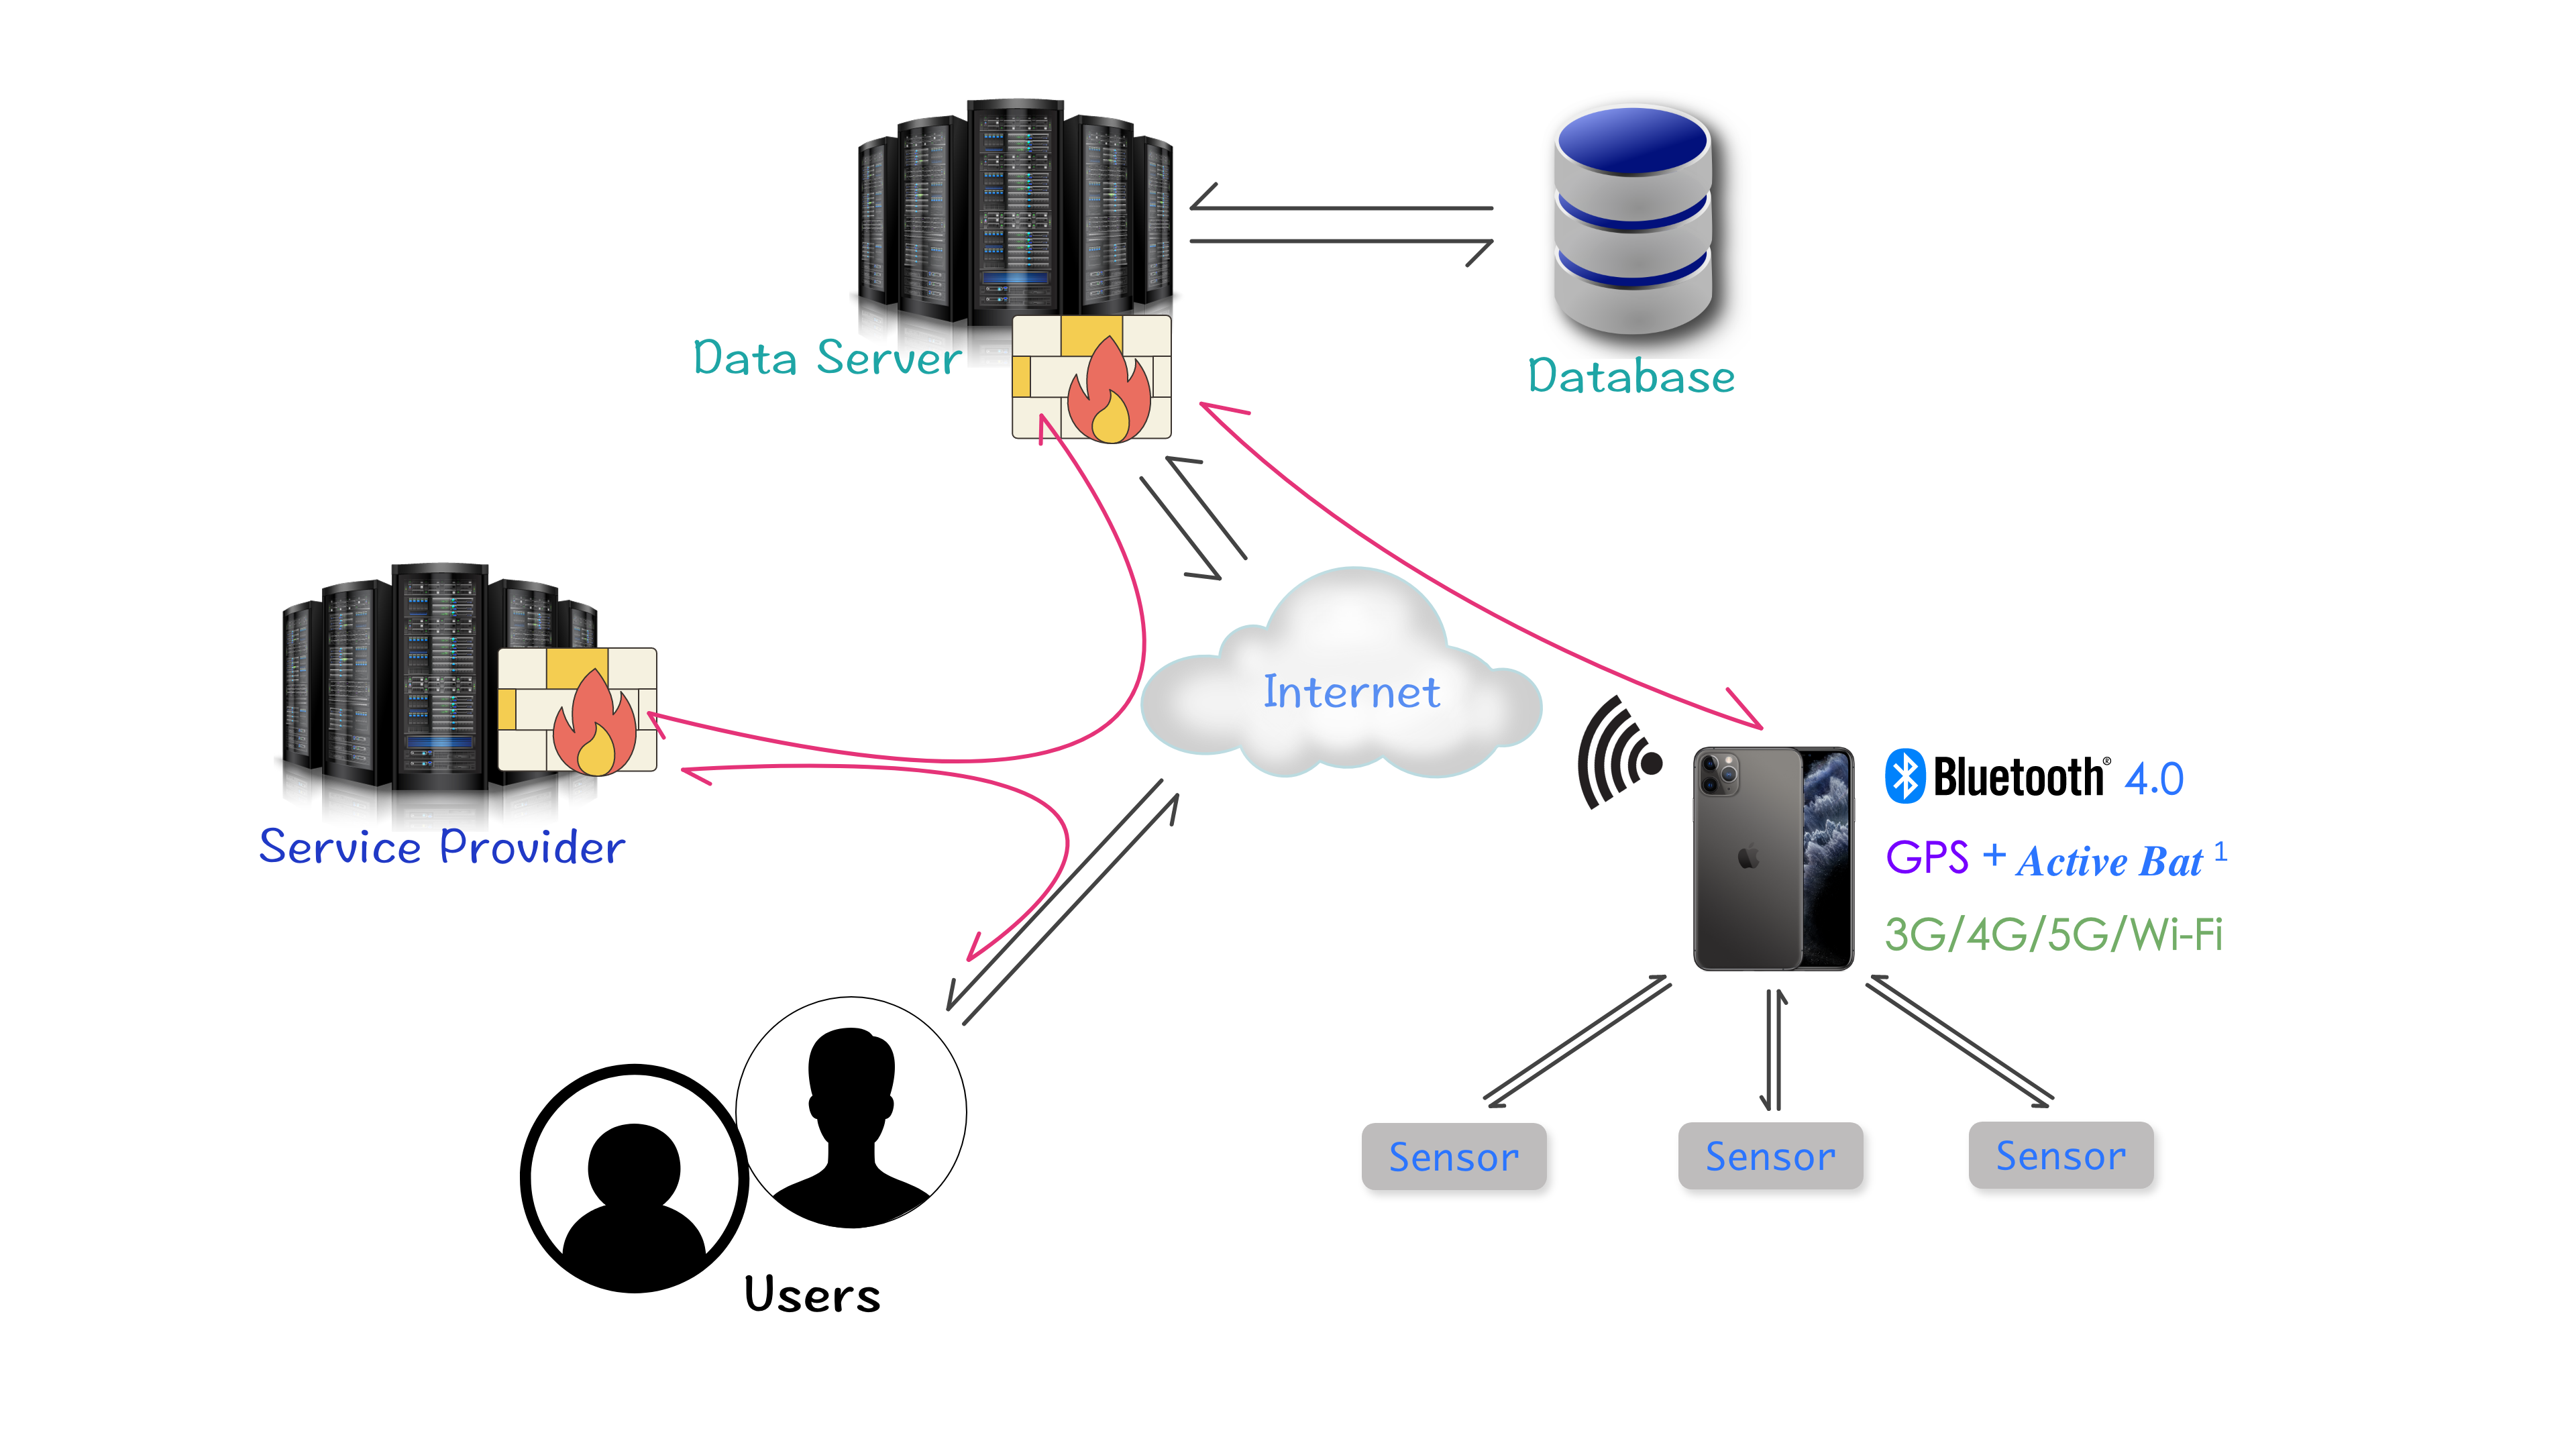
\includegraphics[width=2.5in]{figs/Architecture.png} % 可以是相对路径或者绝对路径,但是由于我们的项目是共享型的,建议使用相对路径,相对本文件
%     \caption{Architecture of the System} % \caption{...} 一定要写在\includegraphics{...}后面,\label{...}写在\caption{...}后面
%     \label{fig_sim}
% \end{figure}

There are multiple options for creating an IoT network: Wi-Fi, Bluetooth, and ZigBee. 
Each of them has its own characteristics. However, in our system, one specific networking 
technology should be chosen to connect the sensors on people's body and the smart device that has 
internet connection via either Wi-Fi or Cellular. Our candidates are:
\begin{itemize}
    
    \item Wi-Fi
    \item Bluetooth Classic
    \item ZigBee
    \item Bluetooth Low Energy(BLE)

\end{itemize}


\subsubsection{Wi-Fi}

\subsubsection{Bluetooth Classic}

\subsubsection{ZigBee}

\subsubsection{Bluetooth Low Energy}

\subsubsection*{System Requirements Analysis}





% Yujie Wang
\subsection{Internet Data Flow}


Your section goes here, Wang.






% Kai Lin
\subsection{Application Layer}

Kai, this is your section, right? \\

\subsubsection{Cloud Computing and Database}



\subsubsection{Other Concerns}






\section{Use Case Scenarios}
Paragraph one Paragraph one Paragraph one Paragraph one Paragraph one 
Paragraph one Paragraph one Paragraph one Paragraph one Paragraph one 
Paragraph one Paragraph one Paragraph one Paragraph one Paragraph one 
Paragraph one Paragraph one Paragraph one Paragraph one Paragraph one 
Paragraph one Paragraph one Paragraph one Paragraph one Paragraph one 

Paragraph two Paragraph two Paragraph two Paragraph two Paragraph two 
Paragraph two Paragraph two Paragraph two Paragraph two Paragraph two 
Paragraph two Paragraph two Paragraph two Paragraph two Paragraph two 
Paragraph two Paragraph two Paragraph two Paragraph two Paragraph two 
Paragraph two Paragraph two Paragraph two Paragraph two Paragraph two 

\section{Conclusion}

Paragraph one Paragraph one Paragraph one Paragraph one Paragraph one 
Paragraph one Paragraph one Paragraph one Paragraph one Paragraph one 
Paragraph one Paragraph one Paragraph one Paragraph one Paragraph one 
Paragraph one Paragraph one Paragraph one Paragraph one Paragraph one 
Paragraph one Paragraph one Paragraph one Paragraph one Paragraph one 

Paragraph two Paragraph two Paragraph two Paragraph two Paragraph two 
Paragraph two Paragraph two Paragraph two Paragraph two Paragraph two 
Paragraph two Paragraph two Paragraph two Paragraph two Paragraph two 
Paragraph two Paragraph two Paragraph two Paragraph two Paragraph two 
Paragraph two Paragraph two Paragraph two Paragraph two Paragraph two 

\section*{Acknowledgments}

Paragraph one Paragraph one Paragraph one Paragraph one Paragraph one 
Paragraph one Paragraph one Paragraph one Paragraph one Paragraph one 
Paragraph one Paragraph one Paragraph one Paragraph one Paragraph one 
Paragraph one Paragraph one Paragraph one Paragraph one Paragraph one 
Paragraph one Paragraph one Paragraph one Paragraph one Paragraph one 

Paragraph three

\bibliographystyle{IEEEtran}
\bibliography{References}
\end{document}